\title{\LARGE{Exercise Sheet 0x02}\\%
\Large{PSI-AdvaSP-M: Advanced Security and Privacy}
}
\author{
Barbara Hoffmann (1759786)\\
Sascha Riechel (1740803)\\
Isabell Sailer (1863490)\\
Tobias Schwartz (1738195)\\
}

\date{Submitted: \today}

\documentclass[12pt]{article}
\usepackage{graphicx}

\begin{document}
\maketitle


\section{Task 1}\label{task1}
\emph{Search for evidence in the pcap file that indicates which kind of web browser was
used by the user?}
In the pcap file we found a packet that uses the Simple Service Discovery Protol, where the USER-AGENT is specified as Google Chrome, as depicted in figure \ref{wireshark_browser}.
\begin{figure}[h]%
\centering%
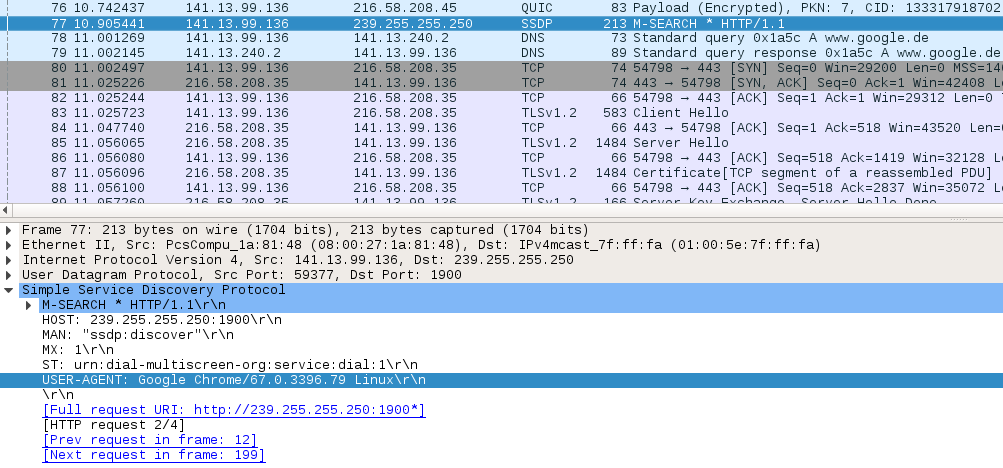
\includegraphics[width=\textwidth]{images/task_1_evidence_browser.png}%
\caption{Wireshark local traffic observation of browser}%
\label{wireshark_browser}%
\end{figure}%



\section{Task 2}\label{task2}
To view only the traffic inside the local network, we employ a display filter in wireshark to show only traffic with destination and source subnet from our own IP-address. Our own IP is most likely 141.13.99.136 and thus we choose 141.13.99.0/24 as subnet filter. This results in only 137 packets which can be seen in Figure~\ref{img_wireshark_overview}.

\begin{figure}[h]%
\centering%
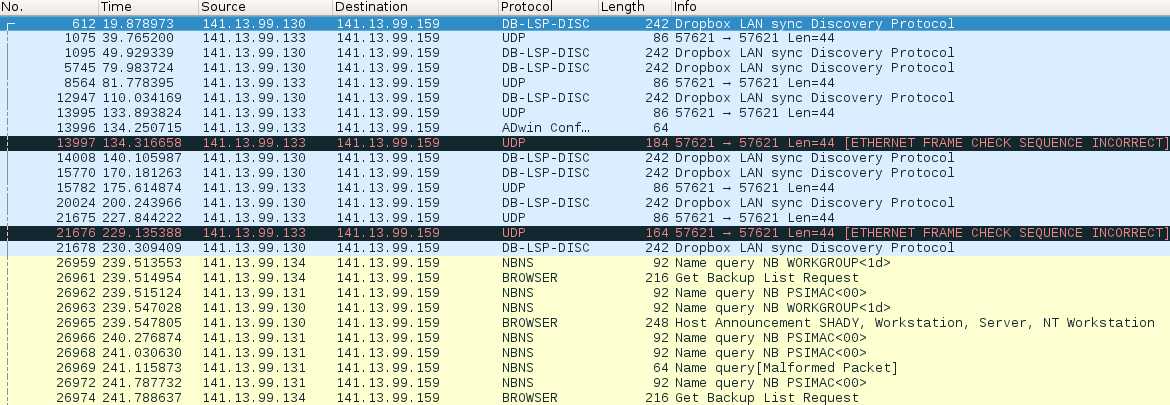
\includegraphics[width=\textwidth]{images/wireshark_overview.png}%
\caption{Wireshark local traffic observation}%
\label{img_wireshark_overview}%
\end{figure}%

% FIGURE 

We can see a dropbox service running and mainly NBNS and BROWSER traffic broadcasted in the local network. As an example we analyze one of the BROWSER pakets (see Figure~\ref{img_wireshark_browser}).
A host with name "SHADY" running Windows 7 or Windows Server 2008 R2 is available on IP-address 141.13.99.130.

\begin{figure}[h]%
\centering%
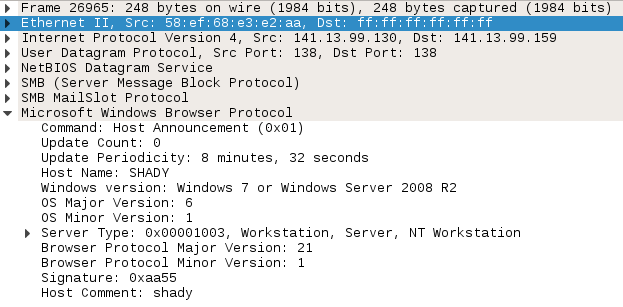
\includegraphics[width=\textwidth]{images/wireshark_browser.png}%
\caption{Wireshark BROWSER packet analysis}%
\label{img_wireshark_browser}%
\end{figure}%

Additionally, we are able to retrieve a GeoIP entry stating that all examined packets were issued in Bamberg by the ``Verein zur Foerderung eines Deutschen Forschungsnetzes e.V." (see Figure~\ref{img_wireshark_geoip}).

\begin{figure}[h]%
\centering%
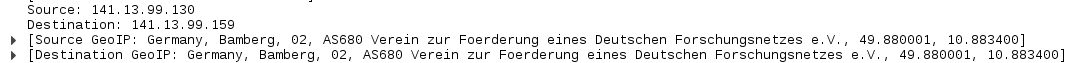
\includegraphics[width=\textwidth]{images/wireshark_geoip.png}%
\caption{Wireshark GeoIp observation}%
\label{img_wireshark_browser}%
\end{figure}%


\section{Task 3}\label{task3}
\end{document}
